\documentclass[../main.tex]{subfiles}
\begin{document}

\chapter{Lecture 12 - 21-04-2020}

\section{Non parametrics algorithms}

We talk about \bred{consistency}: as the training size grows unbounded the expected risk of algorithms converge to Bayes Risk.
\\\\
Now we talk about \bred{non parametric algorithm}: the structure of the model is determined by the data.\\
Structure of the model is fixed, like the structure of a Neural Network but in non parametric algorithm will change structure of the model as the data grows ($\knn$ and tree predictor).\\
If I live the tree grow unboundenly then we get a non parametric tree, but if we bound the grows then we get a parametric one.
\\\\
The converve rate of Bayes Risk (in this case doubled) was small.
Converge of $1$-$NN$ to $2 \, \ell_D(f^*)$ is $m^{-\frac{1}{d+1}}$ so we need an esponential  in the dimension. And we need this is under Lips assumption of $\eta$.
\\ It's possible to converge to Bayes Risk and it's called \bred{No free lunch}.
\subsection{Theorem: No free lunch}
Let a sequenece of number 
$a_1, a_2$ ... $\in \barra{R} $ 
such that they converge to 0. 
\\Also $\frac{1}{22222222} \geq a_1 \geq a_2 \geq ...$ $\forall A $ 
for binary classification $\exists D$ s. t. 
\\$\ell_D(f^*) = 0 $ (zero-one loss) so Bayes risk is zero and 
\expt{\ell_D\left(A(S_M)\right)} $\geq a_m \quad \forall m \geq 1$
\\
Any Bayes Optimal you should be prepared to do so on long period of time. This means that:
\begin{itemize}
\item For specific data distribution $D$, then $A$ may converge fast to Bayes Risk.
\item If $\eta$ is Lipschitz then it is continous. This mean that we perturb the input by the output doesno't change too much.
\item If Bayes Risk is 0 ($\ell_D(f^*) = 0$) function will be discontinous
\end{itemize}
This result typically people think twice for using consistent algorithm because
\begin{figure}[h]
    \centering
    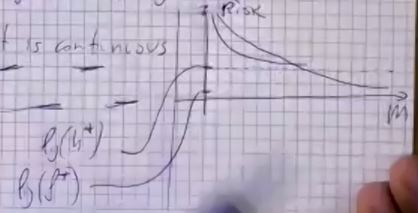
\includegraphics[width=0.6\linewidth]{../img/lez12-img1.JPG}
    \caption{Tree building}
    %\label{fig:}
\end{figure}\\
\\
I have Bayes risk and some non conssitent algorithm that will converge to some value ($\ell_D(\hat{h}^*)$).
Maybe i have Bayes risk and the convergence takes a lot on increasing data points. Before converging was better non parametric (?..)
\\\\
Picture for binary classification, (similar for other  losses)
\begin{itemize}
\item Under no assumption on $\eta$, the typicall "parametric" converge rate to risk of best model in $H$ (including ERM) is $m^{-\frac{1}{2}}$. (Bias error may be high)
\item Under no assumption on $\eta$ there is no guaranteed convergence to Bayes Risk (in general) and this is \bred{no-free-lunch} that guaranteed me no convergence rate.
\item Under Lipshtiz assunption on $\eta$ the typical non parametric convergence to Bayes Risk is $m^{-\frac{1}{d+1}}$. This is exponentially worst than the parametric convergency rate.
\end{itemize}
The exponential depencendece on $d$ is called \bred{Curse of dimnsionality}.
\\ But if I assume small number of dimension $\longrightarrow$ $\knn$ is ok if $d$ is small (and $\eta$ is "easy")
\\
If you have a non parametric algorithm (no Bayes error but may have exponentially infinity training error).
I want them to be balanced and avoid bias and variance. We need to introduce a bit of bias in controlled way.
\\
Inserting bias to reducing variance error. So we sacrify a bit to get a better variance error.
\\\\
It could be good to inject bias in order to reduce the variance error. In practise instead of having 0 training error i want to have a larger training error and hope to reduce overfitting sacrifing a bit in the training error.
\\
I can increase bias in different technics: one is the unsamble methods.


\section{Highly Parametric Learning Algorithm}

\subsection{Linear Predictors}
Our domain is Euclidean space (so we have points of numbers).
\\
$$
X \ is \ \barra{R}^d \qquad x = (x_1,..,x_d)
$$
A linear predictor will be a linear function of the data points.
$$
h: \barra{R}^d \longrightarrow Y \qquad h\left(x\right) = f(w^T \, x) \quad w \in \barra{R}^d
$$
$$
f: \barra{R} \longrightarrow Y
$$
And this is the dot product that is
$$
w^T \, x = \sum_{t = 1}^{d} w_i x_i = \| w \| \, \| x \| \cos \Theta
$$
\begin{figure}[h]
    \centering
    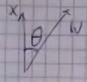
\includegraphics[width=0.2\linewidth]{../img/lez12-img2.JPG}
    \caption{Dot product}
    %\label{fig:}
\end{figure}\\
Suppose we look a regression with square loss.\\
$$ Y = \barra{R} \qquad h(x) = w^T\, x \quad w \in \barra{R}^d
$$
$
f^*(x) = $\expt{ Y| X=x }
\\
Binary classification with zero-one loss 
$ Y = \{ -1,1\}$
We cannot use this since is not a real number but i can do:
$$
h(x) = sgn\left(w^T\, x\right) \qquad sgn(x) = \begin{cases}
+1 \ if \ z > 0\\
-1 \ if \ z \leq 0 
\end{cases}
$$
where sgn is a sign function.
Linear classifier.
\\
$\| X \| \cos \Theta $ is the length of the projection of $x$ onto $w$
\begin{figure}[h]
    \centering
    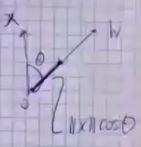
\includegraphics[width=0.2\linewidth]{../img/lez12-img3.JPG}
    \caption{Dot product}
    %\label{fig:}
\end{figure}\\
Now let's look at this set:
$$
\{ x \in \barra{R}^d : w^Tx = c\}
$$
This is a hyperplane.
$$ 
\|w \| \| x \| \cos \Theta = c
\qquad
\|x \| \cos \Theta = \frac{c}{\| w\|}
$$
\begin{figure}[h]
    \centering
    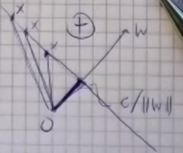
\includegraphics[width=0.4\linewidth]{../img/lez12-img4.JPG}
    \caption{Hyperplane}
    %\label{fig:}
\end{figure}\\
So $ (w,c)$ describe an hyperplane.
\\
We can do binary classification using the hyperplane. Any points that lives in the positive half space and the negative. So the hyperplane is splitting in halfs.
$ H \equiv \{ x \in \barra{R}^d : w^T x = c \}$\
$$
H^+ \equiv \{x \in \barra{R}^d : w^Tx > c \} \qquad \textbf{positive $h_s$}
$$
$$
H^- \equiv \{x \in \barra{R}^d : w^Tx \leq \} \qquad \textbf{negative $h_s$}
$$\
$$ h(x) = 
\begin{cases}
+1 \ if \ x \in H^+\\
-1 \ if \ x \not\in H^-
\end{cases} \qquad
h(x) = sgn (w^T -c)
$$
\begin{figure}[h]
    \centering
    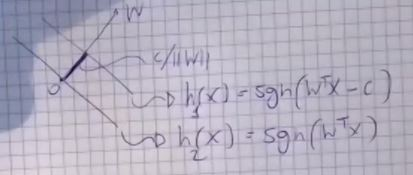
\includegraphics[width=0.6\linewidth]{../img/lez12-img5.JPG}
    \caption{Hyperplane}
    %\label{fig:}
\end{figure}
\newpage
$h_1$ is non-homogenous linear classifier.\\
$h_2$ is homogenous linear classifier.
\begin{figure}[h]
    \centering
    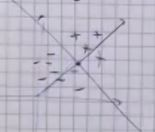
\includegraphics[width=0.3\linewidth]{../img/lez12-img6.JPG}
    \caption{Hyperplane}
    %\label{fig:}
\end{figure}
Any homogenous classifier is equivalent to this:
$$
\{x \in \barra{R}^d : X = c \} \textbf{ is equivalent to \quad} \{x: \barra{R}^{d+1} : \nu^T x = 0 \}
$$
$$
\nu = (w_1,..,w_d, -c) \qquad x' = (x_1,..., x_d, 1)
$$
So we added a dimension.
$$
w^T x = c \ \Leftrightarrow \ \nu^T x' = 0 
$$
$$
\sum_{i} w_1 x_1 = c \ \Leftrightarrow \ \sum_{i} w_1 x_1 -c = 0
$$\\\\
\bred{Rule}:\\
\textbf{When you learn predictor just add an extra feature to your data points, set it ot 1 and forget about non- homogenous stuff.}
\newpage
One dimensional example
\begin{figure}[h]
    \centering
    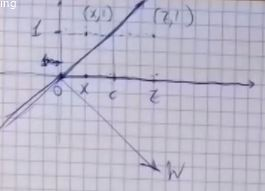
\includegraphics[width=0.6\linewidth]{../img/lez12-img7.JPG}
    \caption{Example of one dimensional hyperplane}
    %\label{fig:}
\end{figure}\\
I have negative (left of $(x,1)$ and positive point (left of $(z,1$) classified 
\\\\
Now i want to learn linear classifier. How can i do it?
$$
H_d = \{ \ h : \exists w \in \barra{R}^d \ h(x) = sgn(w^T x) \ \}
$$
Parametric!
\\
We expect high bias a low variance.
\\
$$
ERM  \qquad \hat{h}_S = arg \min_{h \in H_d} \ \frac{1}{m} \cdot \sum_{t = 1}^{m} I \{h(x_t) \neq y_t \}  = 
$$
$$
= \  arg \min_{w \in \barra{R}^d} \ \frac{1}{m} \cdot \sum_{t = 1}^{m} I \, \{ \, y_t \, w^T x_t \leq 0 \, \} 
$$
A bad optimisation problem!
\\\\
\bred{FACT}:\\
It is unlikely to find an algorithm that solves ERM for $H_d$ and zero-one loss efficiently. 
\\
\bred{NP completeness problems!}
\\ It's very unlikely to solve this problem.
\\
This problem is called \textbf{MinDisagreement}
\\
\subsection{MinDisagreement}
Instance: $(x_1, y_1) ... (x_m, y_m) \in \{ 0,1 \}^d \, x \, \{-1, 1 \}, \quad k \in \barra{N}$\\
Question: Is there $w \in x \, D^d $ \\ s.t $y_t \, w^T   x_t \leq 0$ for at most $k$ indices $t \in \{1,...m\}$
\\
This is NP-complete!
%\expt{\ell(\hat{\ell}) + 2}


\end{document}